%!TEX root = prospectus.tex
%\hl{\\BOOKMARK: PROOFED UP TO HERE\\} 

The term \emph{General Purpose Computing on GPUs} (GPGPU) refers to the application of a Graphics Processing Unit (GPU) 
to problems other than typical rendering tasks (i.e., vertex transformation, rasterization, etc). 

Driven by the gaming industry's insatiable desire for more realistic graphics, GPU performance in the last few years has 
tremendously grown compared to CPUs.
Based on \cite{Jansen:2007, CudaGuide:2008, GTX280:2008, Core2Extreme:2008, FermiPrice:2009}, we see in Figure~
\ref{fig:gpuevolution} the widening gap between compute capabilities on 
the GPU and CPU. The latest GPUs are capable of approximately ten times the number of 
floating point operations per second compared to the latest generation CPU. Naturally, this peak performance comes with limitations: historically GPUs have always lagged behind the CPU in terms 
of flexibility and programmability. For 
example, it was only in 2008, that support for IEEE 754 double precision was added to the GPU \cite{GTX280:2008}. In Chapters~\ref{chap:languages} and \ref{chap:hardware} we will discuss in more depth the history of GPUs and how to utilize them. Here, we concentrate on related work solving  PDEs with meshed methods on clusters of GPUs, and work related to RBFs that has been implemented on GPUs. 
\begin{figure}
      \centering
       \scalebox{0.50}
      { 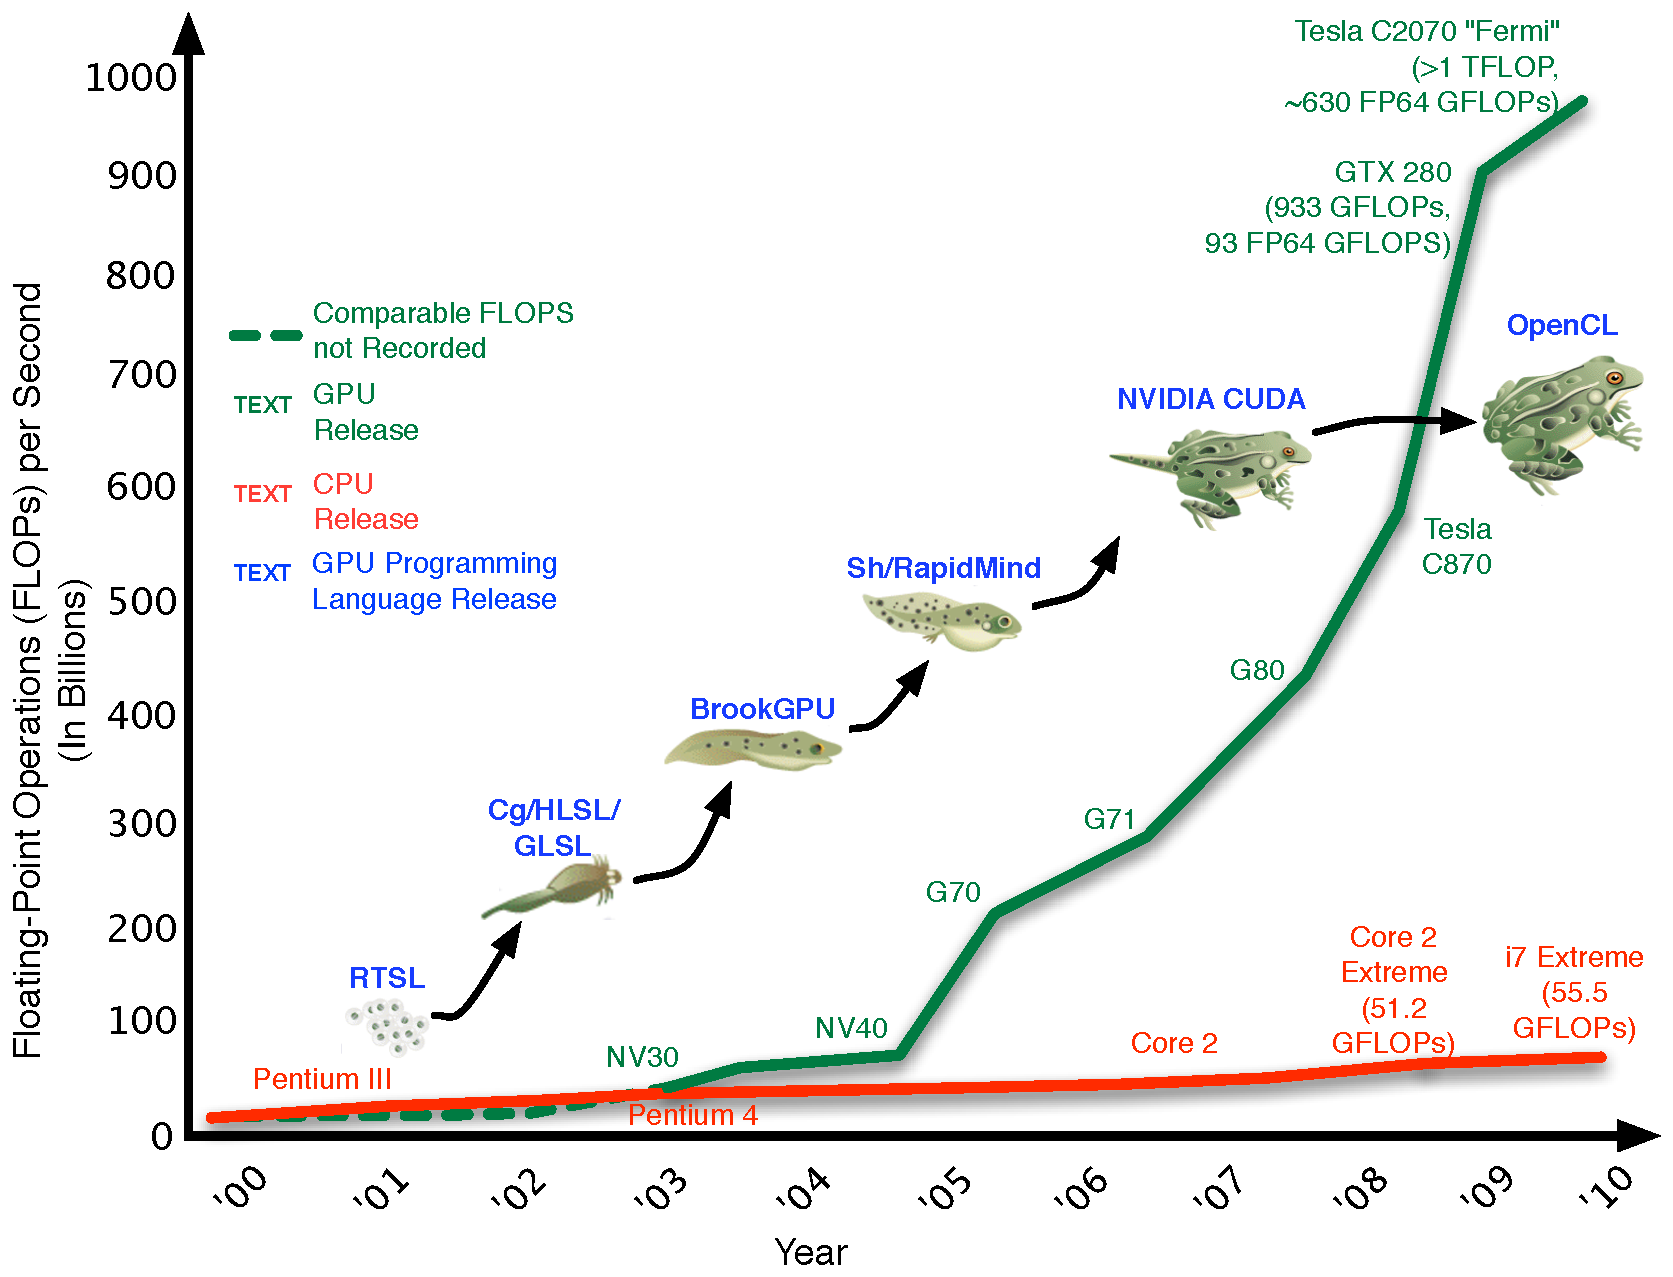
\includegraphics{figures/GPU_Evolution_opencl.pdf}
        \label{fig:gpuevolution}
      }
       \caption{The growing divide between estimated peak performance of CPUs and
        GPUs, joined by landmark releases of maturing languages to control the hardware. Release dates
         of both hardware and languages are approximate. }
%\togordon{I updated the figure. Any comments?} } 
\end{figure}

\subsection{Fluid Simulation on GPUs}

%%Related works have accelerated PDE solutions on GPUs by modifying existing libraries with minimally invasive techniques, as well as by writing a new code. New codes allow for fine tuned adjustment and peak performance, but the modified libraries allow faster turn-around on problems.

Meshed methods have received a large amount of attention from the GPU community. For example, Bolz et al. \cite{Bolz:2003} implemented conjugate gradient and multigrid kernels for 2D FD incompressible fluid simulation using FD on a single GPU.  More recently, a single GPU, multigrid finite-difference based solver was applied to 3D compressible fluid flow (Euler equations) by Elsen et al. \cite{Elsen:2008}. Thibault et al. \cite{Thibault:2009} considered 3D incompressible fluid simulation on structured grids with finite-differencing but on multiple GPUs. 

A finite-volume implementation of the 3D incompressible fluid problem on multiple GPUs was given by Corrigan et al. \cite{Corrigan:2009}. Phillips et al. \cite{Phillips:2009} solved the compressible flow equations on an irregular structured grid with finite-volume using multiple GPUs across multiple nodes (eight quad-core workstations with a total of 32 GPUs). 

A series of articles \cite{Goeddeke:2007, Goeddeke:2008a, Goeddeke:2008b, Goeddeke:2009a}, G\"{o}ddeke et al. presented 
a GPU enhanced version of the parallel multigrid finite element package, FEAST. In \cite{Goeddeke:2007} the authors integrated 
GPUs in a minimally invasive fashion (e.g., farming out local multigrid tasks to the GPU) and considered the weak scalability (i.e., 
increasing the number of co-processors while keeping the problem size fixed on each processor) on up to 160 compute nodes with a 
single GPU each.  Since the accelerated routines were implemented below the original FEAST API, it was demonstrated in 
\cite{Goeddeke:2008a} that existing applications built on top of the original FEAST could benefit without code modifications when 
the 
new package, FEASTGPU, was substituted. \cite{Goeddeke:2008b} compared performance of single-,  double- and 
mixed-precision calculation within FEASTGPU. \cite{Goeddeke:2009a} applied FEASTGPU to nonlinear Navier-Stokes 
problems and 
found the minimally invasive approach had limited impact on performance in the new setting where computational work was no longer  
concentrated in GPU-accelerated tasks. 


\subsection{RBFs on GPUs}

While much work on RBFs has been done on GPUs, most of it relates to visualization (e.g., \cite{Cuntz:2007, Weiler:2005}),  surface reconstruction (e.g., \cite{Corrigan:2005,Carr:2003}), and neural networks (e.g., \cite{Brandstetter:2008}). Gumerov, Duraiswami and Dorland \cite{Gumerov:2007a, Gumerov:2007b} tested their library of FORTRAN wrappers for CUDA in implementations of both a pseudospectral plasma turbulence problem (nonlinear PDE), and a fast multipole method for RBF interpolation; they did not solve PDEs with RBFs. 

The only known GPGPU applications of RBFs for PDEs came from our collaborators in Minnesota. In \cite{Schmidt:2009a, Schmidt:2009b}, Schmidt et al. compare GPU implementations of global RBF collocation to a staggered leapfrog FD scheme applied to the 2D (heightfield) shallow water equations for Tsunami simulation. For both methods, time-stepping is controlled by a $4^{th}$ order Runge-Kutta scheme. Results for a problem size of $32\times32$ RBF centers show similar error to a $185\times 185$ staggered leapfrog discretization \cite{Schmidt:2009b}.

Our collaborators wrote their code in MATLAB using AccelerEyes Jacket \cite{JacketGuide:2009} on a single graphics card. While the Jacket library allows for fast prototyping using MATLAB notation on GPU arrays, it does not allow developer control of CPU-GPU communication or compute order (e.g., all operations are synchronous with no overlapping computation and communication). Thus, the efficiency is restricted. 

To clearly distinguish our approach from theirs, we will: 

\cbox{black}{light-gray}{
\begin{itemize}
	\item use GPU languages (CUDA and OpenCL) to implement efficient (optimized) kernels;
	\item use local RBF (collocation and RBF-FD) schemes;
	\item span multiple GPUs on a heterogeneous compute cluster with one or more GPUs per CPU;
	\item utilize asynchronous commands on the GPU to overlap communication and computation for increased efficiency;
%	\item extend simulation into 3D to track horizontal fluid motion;
	\item solve very large problem sizes (several millions of nodes);
	%\item apply the RBF-QR method to test the limit $\varepsilon \rightarrow 0$ for spectral accuracy.
\end{itemize}
}
